
\chapter[Bài tập: Mạch điện xoay chiều có tần số biến thiên]{Bài tập: Mạch điện xoay chiều có tần số biến thiên}
\section{Lý thuyết}
\subsection{Ứng dụng của hiện tượng cộng hưởng điện trong các bài toán về tần số biến thiên}
\subsubsection{Điều kiện xảy ra hiện tượng cộng hưởng điện khi $\omega$ thay đổi}
Để xảy ra hiện tượng cộng hưởng điện thì $Z_L = Z_C$, khi đó giá trị của tần số góc $\omega_0$ là
\begin{equation*}
	\omega_0=\dfrac{1}{\sqrt{LC}}.
\end{equation*}
\subsubsection{Có hai giá trị $\omega_1$, $\omega_2$ cho cùng một giá trị $I$, $\calP$. Tìm tần số góc $\omega_0$ để trong mạch xảy ra hiện tượng cộng hưởng điện}
\begin{align*}
	I_1 &= I_2 \\
	\Leftrightarrow \dfrac{U}{\sqrt{R^2 + (Z_{L1}-Z_{C1})^2}}&=\dfrac{U}{\sqrt{R^2+(Z_{L2}-Z_{C2})^2}}\\
	\Rightarrow (Z_{L1}-Z_{C1})&=-(Z_{L2}-Z_{C2})\\
	\Leftrightarrow L\omega_1 - \dfrac{1}{\omega_1 C} &= -\left(L\omega_2-\dfrac{1}{\omega_2C}\right) \\
	\Leftrightarrow	L(\omega_1+\omega_2)&=\dfrac{1}{C}\left(\dfrac{1}{\omega_1}+\dfrac{1}{\omega_2}\right) \\
	\Leftrightarrow L(\omega_1+\omega_2)&=\dfrac{1}{C}\dfrac{\omega_1+\omega_2}{\omega_1\omega_2} \\
	\Rightarrow \omega_1\omega_2&=\dfrac{1}{LC}=\dfrac{1}{\omega_0^2}.
\end{align*}

Vậy khi $\omega_0=\sqrt{\omega_1\omega_2}$ thì trong mạch xảy ra hiện tượng cộng hưởng điện.
\subsection{Ứng dụng phương pháp đại số trong các bài toán về tần số góc biến thiên}

\subsubsection{Tìm giá trị $\omega$ để điện áp hiệu dụng giữa hai đầu cuộn cảm là lớn nhất ($U_{L\ \text{max}}$)}

Từ công thức tính điện áp hiệu dụng giữa hai đầu cuộn cảm:
\begin{equation*}
	U_L=IZ_L=\dfrac{UZ_L}{\sqrt{R^2+(Z_L-Z_C)^2}},
\end{equation*}
chia cả tử và mẫu cho $\omega L$, ta được:
\begin{equation*}
	U_L=\dfrac{U}{\sqrt{\dfrac{R^2}{\omega^2 L^2}+\dfrac{\omega^2 L^2 - 2 \dfrac{L}{C}+\dfrac{1}{\omega^2 C^2}}{\omega^2 L^2}}}=\dfrac{U}{\sqrt{\dfrac{R^2}{\omega^2 L^2}+\left(1-\dfrac{1}{\omega^2 LC}\right)^2}}.
\end{equation*}
Giá trị $U_L$ lớn nhất khi $\left[\dfrac{R^2}{\omega^2 L^2}+\left(1-\dfrac{1}{\omega^2 LC}\right)^2\right]$ nhỏ nhất.

Đặt $x=\dfrac{1}{\omega^2 L}$ và $y=\dfrac{R^2x}{L}+\left(1-\dfrac{x}{C}\right)^2$.
Lấy đạo hàm của $y$ theo $x$, ta được:
\begin{equation*}
	y'(x)=\dfrac{R^2}{L}-\dfrac{2}{C}\left(1-\dfrac{x}{C}\right).
\end{equation*}
Cho $y'(x)=0$, ta được:
\begin{equation*}
	x=\dfrac{2LC-R^2C^2}{2L}.
\end{equation*}
Vì $x>0 \Rightarrow \dfrac{2L}{C}>R^2$, khi đó ta được bảng biến thiên:
\begin{center}
	\begin{tikzpicture}
		\tkzTab
		[lgt=2,espcl=4,nocadre] % tùy chọn- 2 là độ rộng cột 1 (2cm), 4 là độ rộng giữa 2 giá trị ở hàng 1 cột 2
		{$x$/1,$y'(x)$/1,$y(x)$/2.5} % cột đầu tiên
		{0,$\dfrac{2LC-R^2C^2}{2L}$,$+\infty$} % hàng 1 cột 2
		{,$-$,0,$+$,} % hàng 2 cột 2
		{+/ ,-/$y_{\min}$,+/ } % hàng 3 cột 2
		% lưu ý: kể từ hàng 2 trở đi của cột 2 thì số lượng thành phần nhiều hơn hàng 1 cột 2 do có tính cả các khoảng giữa các giá trị hàng 1.
	\end{tikzpicture}
\end{center}
Thay $x=\dfrac{1}{\omega^2L} = \dfrac{2LC-R^2C^2}{2L}$, ta được bình phương của tần số góc là
\begin{equation*}
	\omega^2 = \dfrac{2}{2LC-R^2C^2}
\end{equation*}
và giá trị của $U_{L\ \text {max}} $ khi đó là
\begin{equation*}
	U_{L\ \text{max}}=\dfrac{2UL}{R\sqrt{4LC-R^2C^2}}.
\end{equation*}
\subsubsection{Tìm giá trị $\omega$ để điện áp giữa hai đầu tụ điện là lớn nhất $(U_{C\ \text{max}})$}
Qua các bước chứng minh (như trên), ta được bình phương của tần số góc là
\begin{equation*}
	\omega^2 = \dfrac{1}{LC}-\dfrac{R^2}{2L^2}
\end{equation*}
và giá trị của $U_{C\ \text {max}} $ khi đó là
\begin{equation*}
	U_{C\ \text{max}}=\dfrac{2UL}{R\sqrt{4LC-R^2C^2}}.
\end{equation*}
\luuy{Nếu cuộn cảm có điện trở $r$ thì
	
	$$U_{C\ \text{max}}=U_{L\ \text{max}}=\dfrac{2UL}{(R+r)\sqrt{4LC-(R+r)^2C^2}}$$}

\section{Mục tiêu bài học - Ví dụ minh họa}
\begin{dang}{Ứng dụng của hiện tượng cộng hưởng điện trong các bài toán về tần số biến thiên}
	\viduii{3}{
		Mạch điện $R_1$, $L_1$, $C_1$ có tần số góc cộng hưởng là $\omega_1$ và mạch $R_2$, $L_2$, $C_2$ có tần số góc cộng hưởng là $\omega_2$, với $\omega_2 = \omega_1$. Nếu mắc nối tiếp hai mạch điện này với nhau thì mạch sẽ cộng hưởng ở tần số góc là
		\begin{mcq}(4)
			\item $\omega=0$.
			\item $\omega=\omega_1$.
			\item $\omega=2\omega_1$.
			\item $\omega=3\omega_1$.
		\end{mcq}
	}
	{\begin{center}
			\textbf{Hướng dẫn giải}
		\end{center}
		
		Các tần số góc cộng hưởng có giá trị:
		\begin{equation*}
			\omega_1 = \dfrac{1}{\sqrt{L_1C_1}}; \omega_2 = \dfrac{1}{\sqrt{L_2C_2}}.
		\end{equation*}
		
		Do $\omega_1 = \omega_2$, nên suy ra
		\begin{align*}
			L_1C_1 &= L_2C_2\\
			\Leftrightarrow L_2&=\dfrac{L_1C_1}{C_2}\\
		\end{align*}
		
		Độ tự cảm và điện dung lúc sau lần lượt là
		\begin{equation*}
			L=L_1+L_2; C=\dfrac{C_1C_2}{C_1+C_2}.
		\end{equation*}
		
		Để mạch xảy ra cộng hưởng điện thì tần số góc có giá trị:
		\begin{equation*}
			\omega=\dfrac{1}{\sqrt{LC}}=\dfrac{1}{\sqrt{(L_1+L_2)\dfrac{C_1C_2}{C_1+C_2}}}
		\end{equation*}
		
		Biến đổi biểu thức dưới dấu căn, ta được:
		\begin{equation*}
			(L_1+L_2)\dfrac{C_1C_2}{C_1+C_2}=\dfrac{\left(L_1+\dfrac{L_1C_1}{C_2}\right)C_1C_2}{C_1+C_2}=\dfrac{L_1\left(1+\dfrac{C_1}{C_2}\right)C_1C_2}{C_1+C_2}=\dfrac{L_1(C_1+C_2)C_1}{C_1+C_2}=L_1C_1
		\end{equation*}
		
		Vậy:
		\begin{equation*}
			\omega=\dfrac{1}{\sqrt{L_1C_1}}=\omega_1.
		\end{equation*}
		
		\textbf{Đáp án: B.}
	}
	\viduii{3}{Cho mạch điện xoay chiều $RLC$ mắc nối tiếp, đặt vào hai đầu đoạn mạch điện áp xoay chiều có biểu thức $u=U_0 \cos 2\pi f t \ \text{V}$ tần số dòng điện thay đổi được. Khi tần số dòng điện là $f_0 = 50\ \text{Hz}$ thì công suất tiêu thụ trên mạch là lớn nhất, khi tần số dòng điện là $f_1$ hoặc $f_2$ thì mạch tiêu thụ cùng công suất $\calP$. Biết $f_1 +f_2 =145\ \text{Hz}$ ($f_1<f_2$), tần số $f_1, f_2$ lần lượt là
		\begin{mcq}(2)
			\item 45 Hz; 100 Hz.
			\item 25 Hz; 120 Hz.
			\item 50 Hz; 95 Hz.
			\item 20 Hz; 125 Hz.
		\end{mcq}	
	}
	{\begin{center}
			\textbf{Hướng dẫn giải}
		\end{center}
		
		Khi công suất tiêu thụ trên mạch lớn nhất thì xảy ra cộng hưởng.
		
		Ta có công thức liên hệ giữa tần số:
		
		$$\omega_0 =\sqrt{\omega^2_1\omega^2_2} \Rightarrow f_0^2=f_1f_2.$$
		
		Kết hợp với đề bài $f_1 +f_2 =145\ \text{Hz}$ ta tính được:
		
		$$f_1 = 20\ \text{Hz}; f_2 =125\ \text{Hz}.$$
		
		\textbf{Đáp án: D.}
		
	}
\end{dang}

\begin{dang}{Ứng dụng phương pháp đại số\\ trong các bài toán về tần số góc biến thiên}
	\viduii{3}{Một đoạn mạch không phân nhánh gồm điện trở thuần $R = 100\ \Omega$ , cuộn dây có độ tự cảm $L = \text{12,5}\ \text{mH}$, tụ điện có điện dung $C = 1\ \mu \text{F}$ . Đặt vào 2 đầu đoạn mạch một điện áp xoay chiều có giá trị hiệu dụng 200 V và có tần số thay đổi được. Thay đổi $f$ để giá trị điện áp hiệu dụng trên cuộn cảm đạt cực đại. Giá trị đó là
		\begin{mcq}(4)
			\item 250 V.
			\item 200 V.
			\item 150 V.
			\item 100 V.
		\end{mcq}
	}
	{\begin{center}
			\textbf{Hướng dẫn giải}
		\end{center}
		Áp dụng công thức điều kiện để điện áp hiệu dụng trên cuộn cảm đạt cực đại, ta có:
		
		$$U_{L\ \text{max}}=\dfrac{2UL}{R\sqrt{4LC-R^2C^2}} = 250\ \text{V}.$$
		
		\textbf{Đáp án: A.}
	}
	\viduii{3}{Đoạn mạch nối tiếp AB gồm tụ điện có điện dung $C = \dfrac{1}{6\pi}\ \text{mF}$ , cuộn cảm có độ tự cảm $L = \dfrac{\text{0,3}}{\pi}\ \text{H}$ , có điện trở $r = 10\ \Omega$ và một biến trở $R$. Đặt vào điện áp xoay chiều có tần số thay đổi được. Khi $f = 50\ \text{Hz}$, thay đổi $R$ thì điện áp hiệu dụng trên tụ đạt cực đại là $U_1$. Khi $R = 30\ \Omega$, thay đổi $f$ thì điện áp hiệu dụng trên tụ cực đại là $U_2$. Tỉ số $\dfrac{U_1}{U_2}$ bằng:
		\begin{mcq}(4)
			\item 1,58.
			\item 3,15.
			\item 0,79.
			\item 6,29.
		\end{mcq}
	}
	{\begin{center}
			\textbf{Hướng dẫn giải}
		\end{center}
		Dung kháng và cảm kháng có giá trị:
		$$Z_C = \dfrac{1}{C\omega} = 60\ \Omega; Z_L =L\omega = 30\ \Omega.$$
		
		Khi $f=50\ \text{Hz}$, thay đổi $R$:
		
		$$U_C =IZ_C =\dfrac{UZ_C}{\sqrt{(R+r)^2 +(Z_L-Z_C)^2}}.$$
		
		Để $U_{C_\text{max}}$ thì $\sqrt{(R+r)^2 +(Z_L-Z_C)^2}$ phải min suy ra $R=0$.
		
		Vậy $$U_{C_\text{max}} = U_1 = \text{0,6}\sqrt{10} U.$$
		
		Khi $R=30\ \Omega$, thay đổi $f$ để $U_{C_\text{max}}$
		
		$$U_{C\ \text{max}}= U_2=\dfrac{2UL}{(R+r)\sqrt{4LC-(R+r)^2C^2}} = \dfrac{\text{4,5}U}{\sqrt {14}}.$$
		
		Do đó:
		$$\dfrac{U_1}{U_2} = \text{1,58}.$$
		
		\textbf{Đáp án: A.}
		
	}
\end{dang}
